\documentclass{experimentreport}

\input{listing_style.tex}

%========================
% Basic Information
%========================

\setcoursename{Intelligence Leading the Frontier, Computing Shaping the Future}
\setreportname{HIT Code Review Research Experiment Report}

\setexperimenttitle{Mining Code Review Comments and Understanding Requirements}

\setstudentname{Ulugbek Khamidov, Komil Tokhirov}
\setdepartment{HITCodeReviewResearch}
\setstudentid{2026140348, 2026140354}

\setcourseteacher{Liu Jiakun}
\setinstructor{Liu Jiakun}

\setlablocation{HIT First Campus}
\setlabtime{2024-06-11 14:00-17:00}

\begin{document}

\makereporthead

\experimentpurpose{
- Understood traditional machine learning workflow for code review.
- Mastered data preprocessing for code review tasks.
- Extracted AST and CFG representations from code.
- Extracted structural, textual, and statistical features.
- Trained SVM and Random Forest models.
- Built a merge prediction model and analyzed performance.
}

\experimentcontent{
- Filtered 1,020 human-written PRs from Experiment 1 dataset.
- Extracted AST representations using Python's ast module.
- Extracted CFG representations for control flow analysis.
- Extracted 9 features: additions, deletions, changed\_files, commits\_count, reviewers\_count, comments\_count, labels\_count, pr\_length, has\_ai\_reviewer.
- Constructed ML dataset: 816 train, 204 test.
- Trained SVM (RBF kernel) and Random Forest (100 trees).
- Evaluated using accuracy, precision, recall, F1, ROC-AUC.
}

\experimentresult{
We trained SVM and Random Forest on 1,020 human-written PRs (601 merged, 419 not merged).

SVM Results:
- Accuracy: 88.7\%
- Precision: 88.2\%
- Recall: 93.3\%
- F1: 90.7\%
- ROC-AUC: 92.3\%

Random Forest Results:
- Accuracy: 91.2\%
- Precision: 88.6\%
- Recall: 97.5\%
- F1: 92.9\%
- ROC-AUC: 97.3\%

Random Forest outperformed SVM across all metrics. Feature importance analysis showed labels\_count (45.3\%) as the dominant predictor, followed by pr\_length (12.2\%) and deletions (10.3\%).

AST and CFG examples were generated for sample code snippets.
}

%========================
% Figures Section (Before Instructor Comments)
%========================

\section*{Figures}


\begin{figure}[h]
\centering
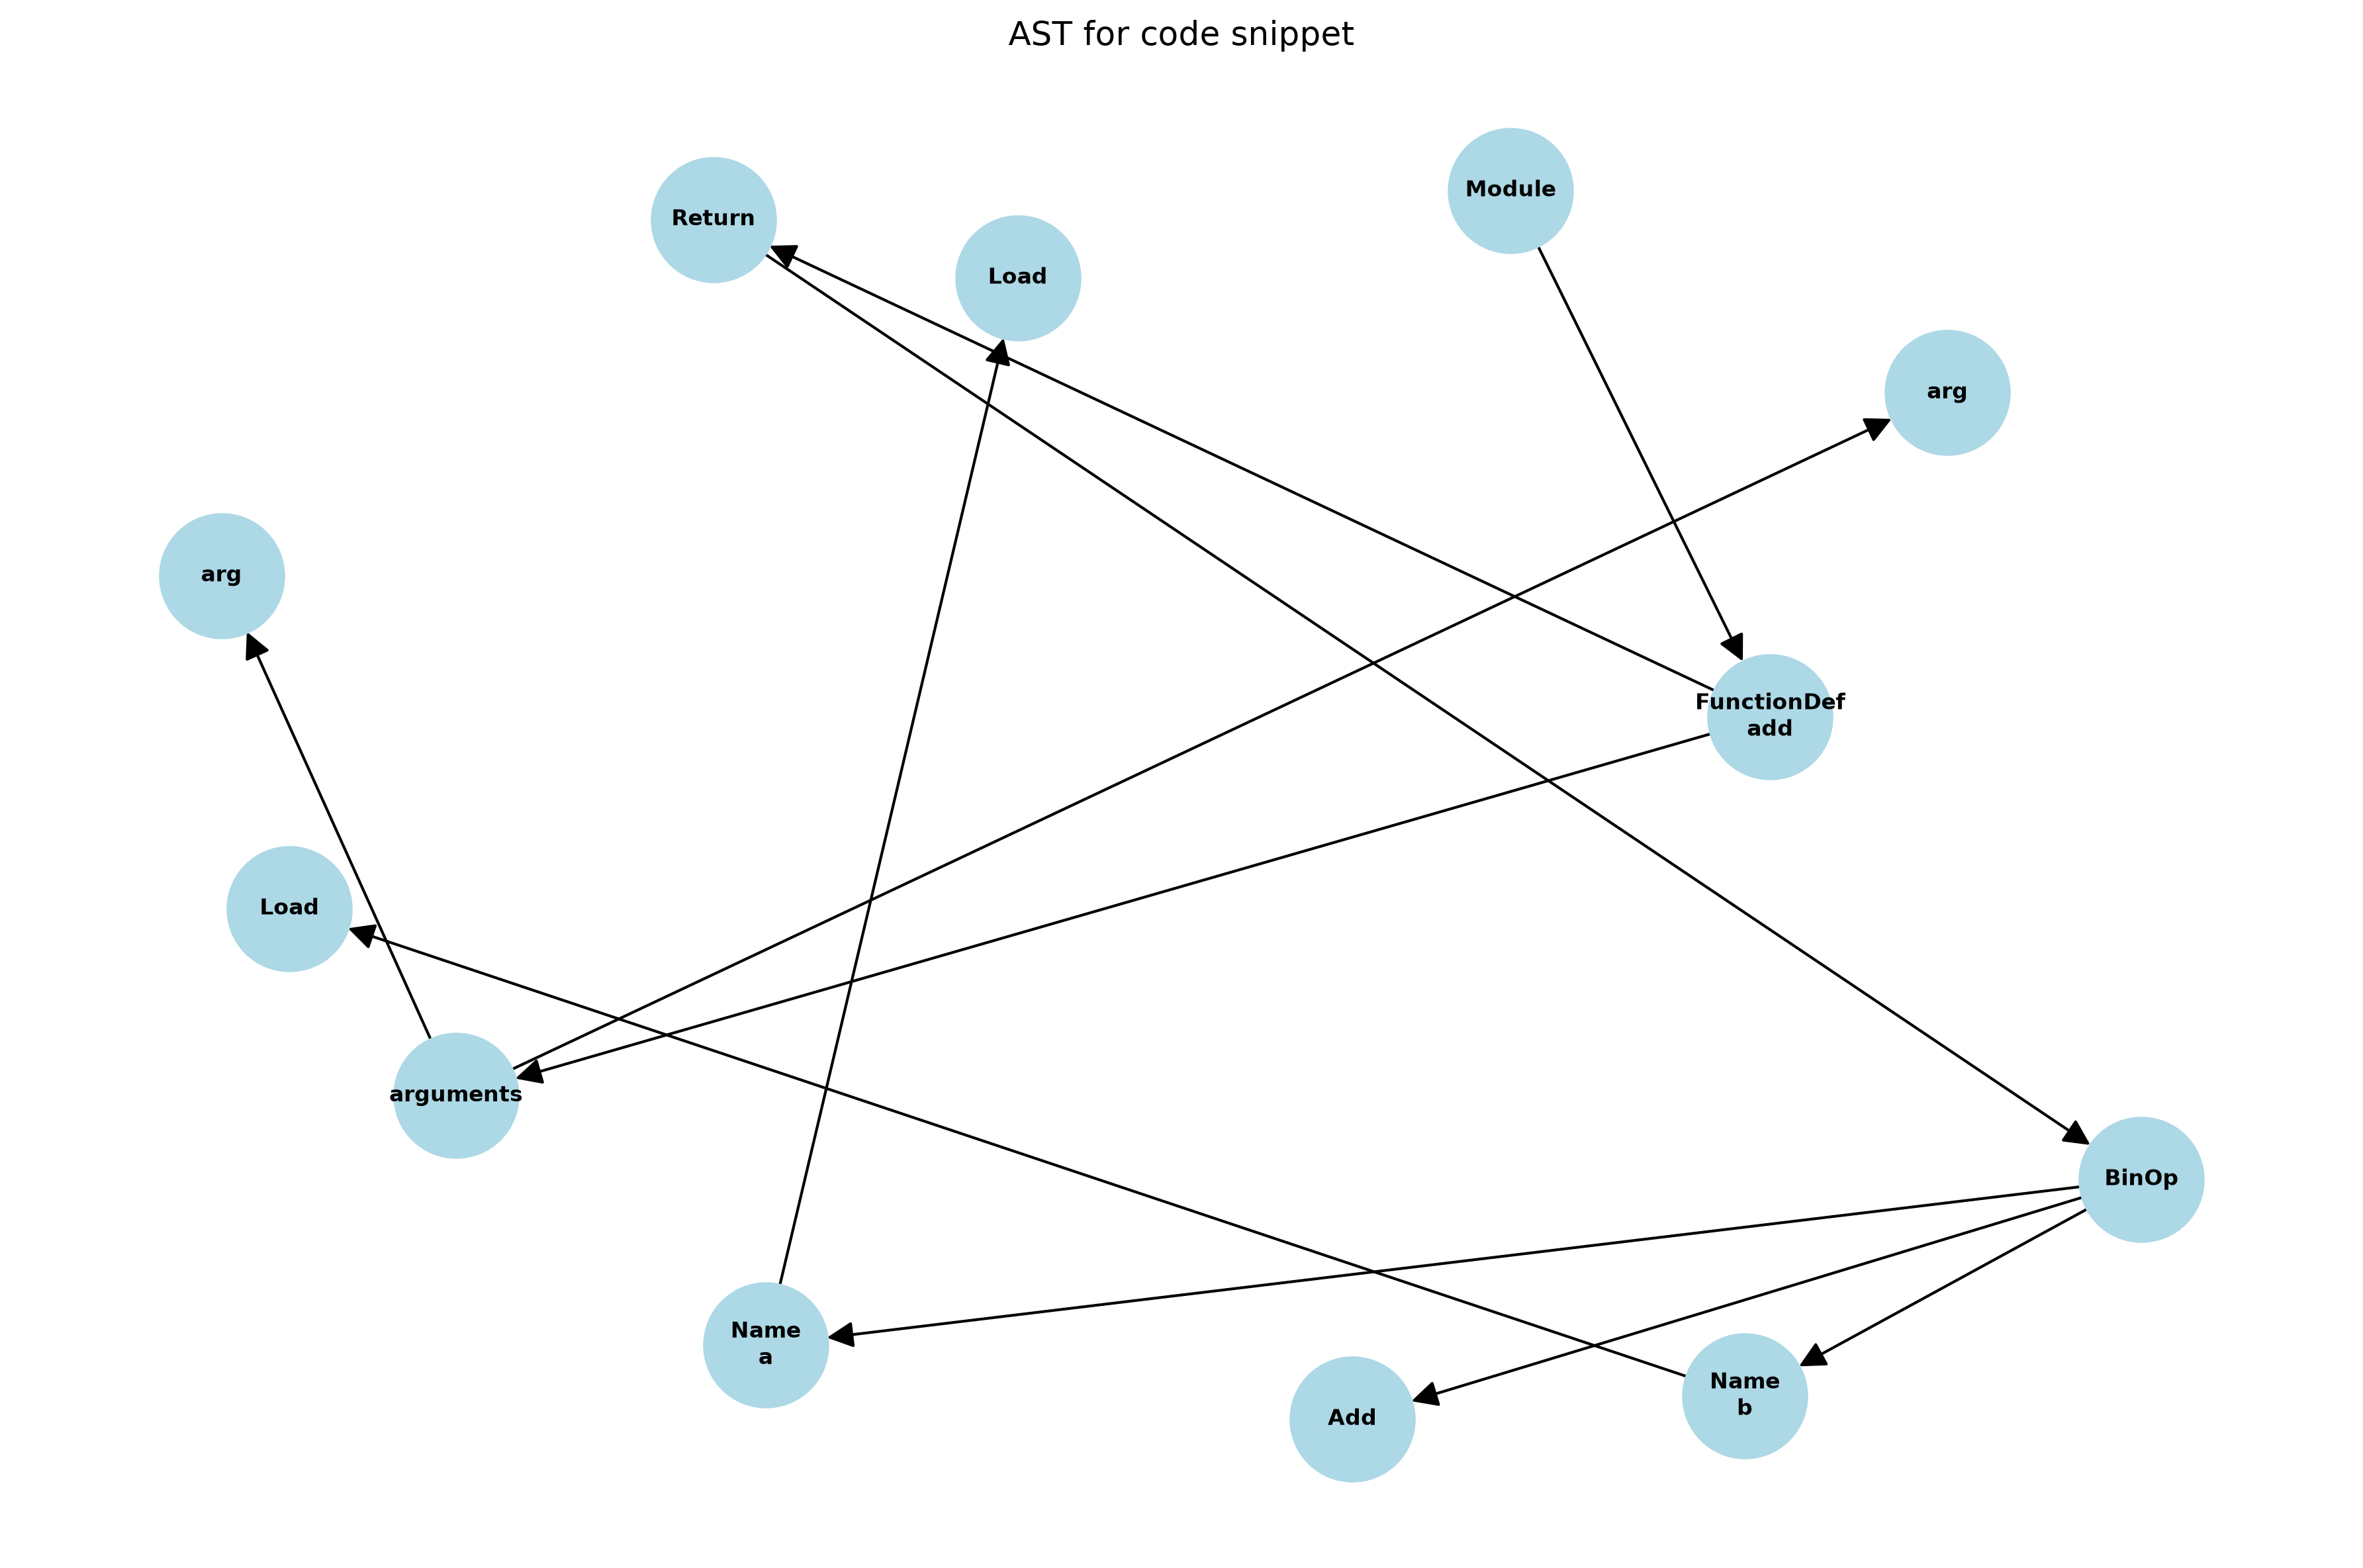
\includegraphics[width=0.8\textwidth]{ast_sample_1.png}
\caption{AST for a simple addition function}
\end{figure}

\begin{figure}[h]
\centering
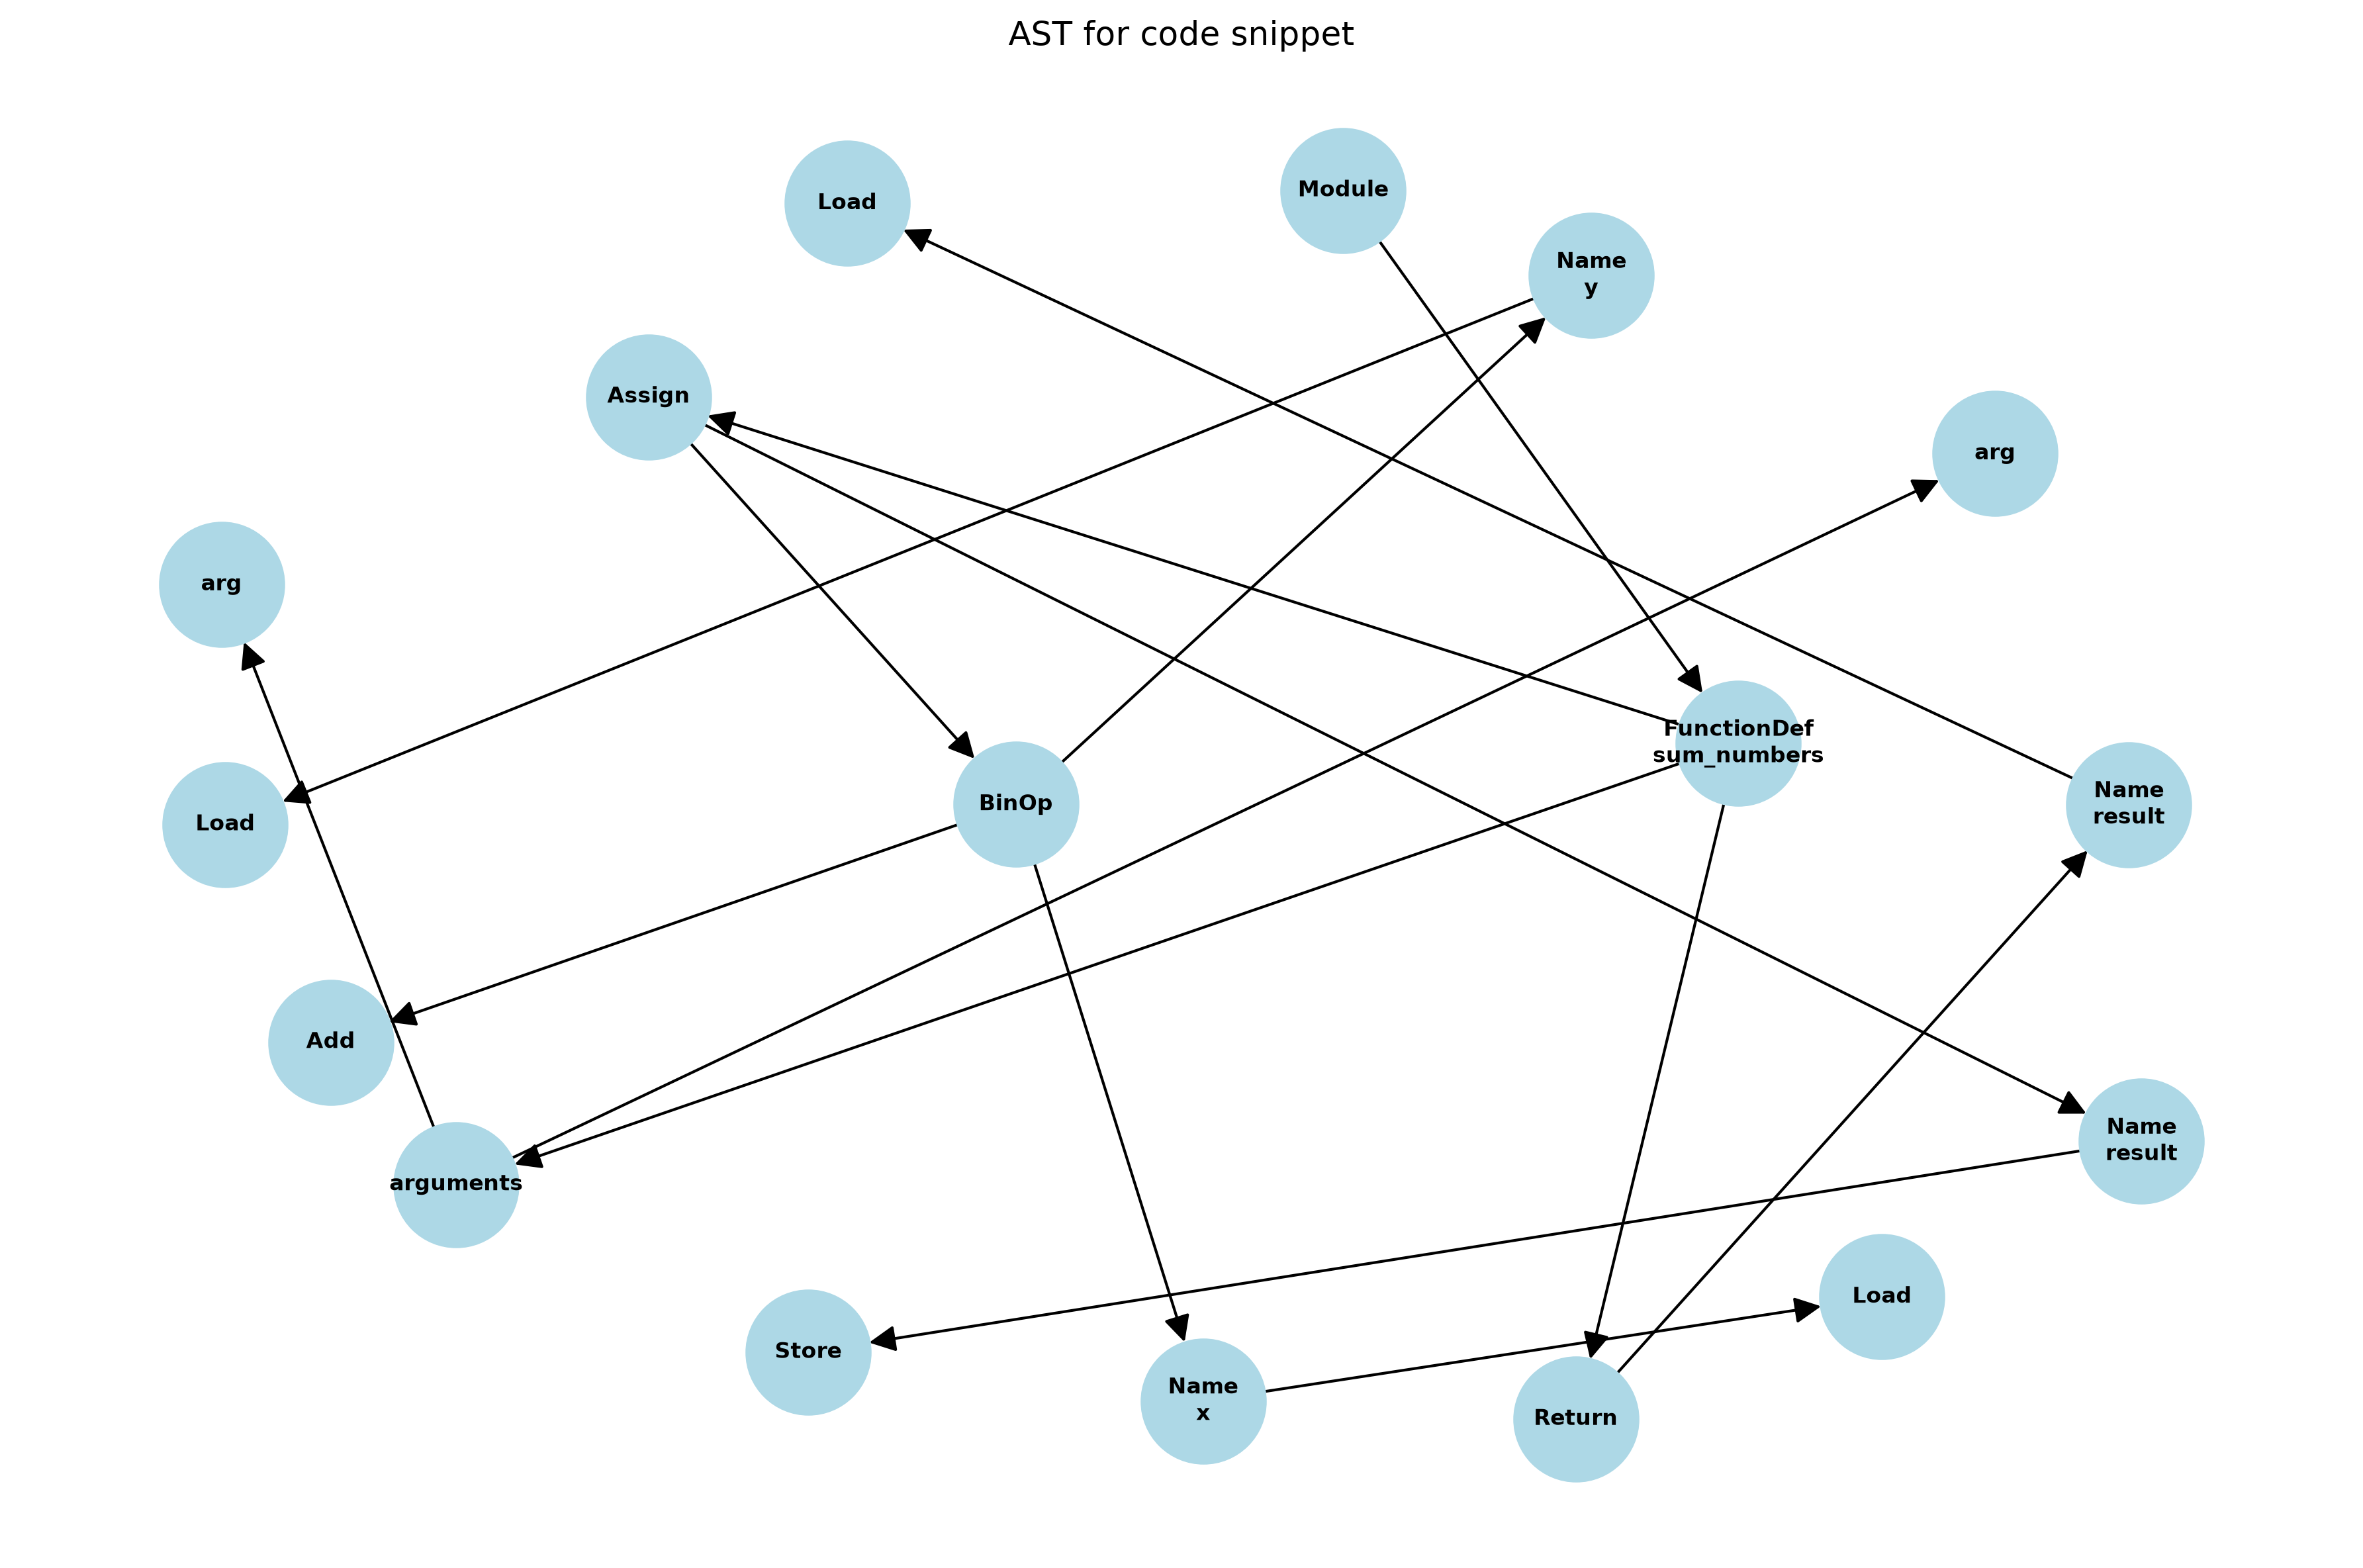
\includegraphics[width=0.8\textwidth]{ast_sample_2.png}
\caption{AST for a function with intermediate variable}
\end{figure}

\begin{figure}[h]
\centering
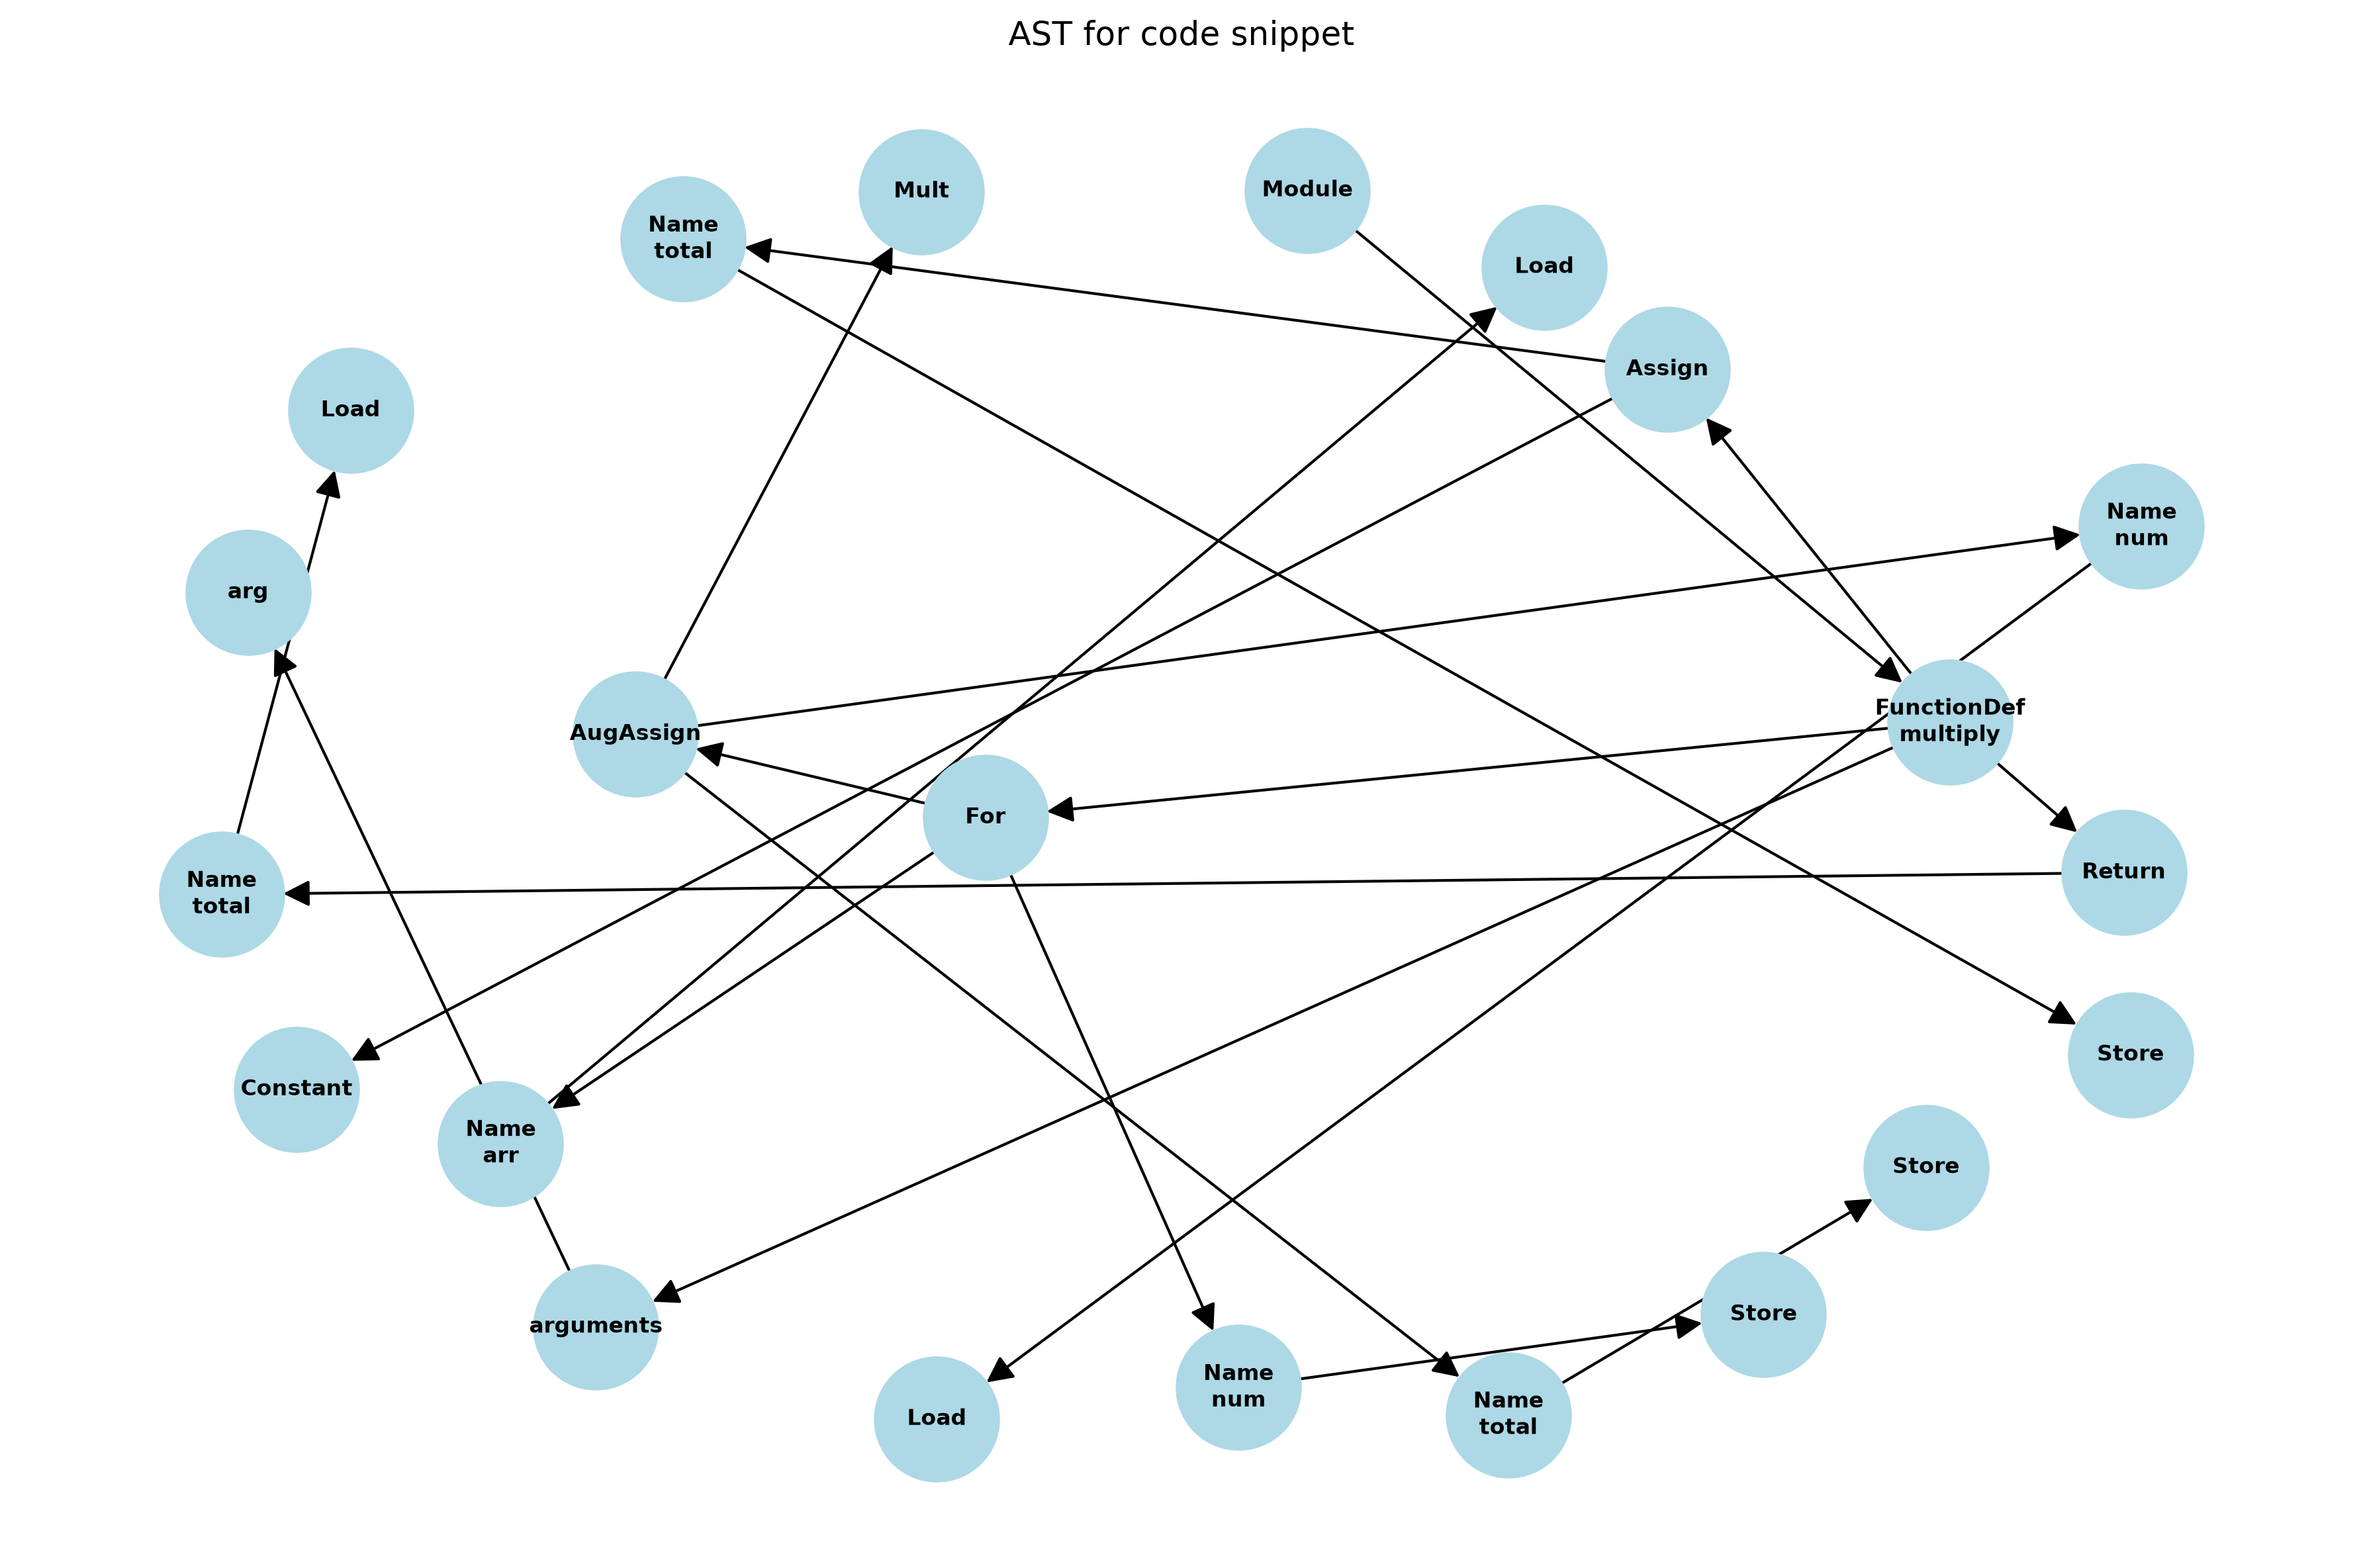
\includegraphics[width=0.8\textwidth]{ast_sample_3.png}
\caption{AST for a function with loop}
\end{figure}


\begin{figure}[h]
\centering
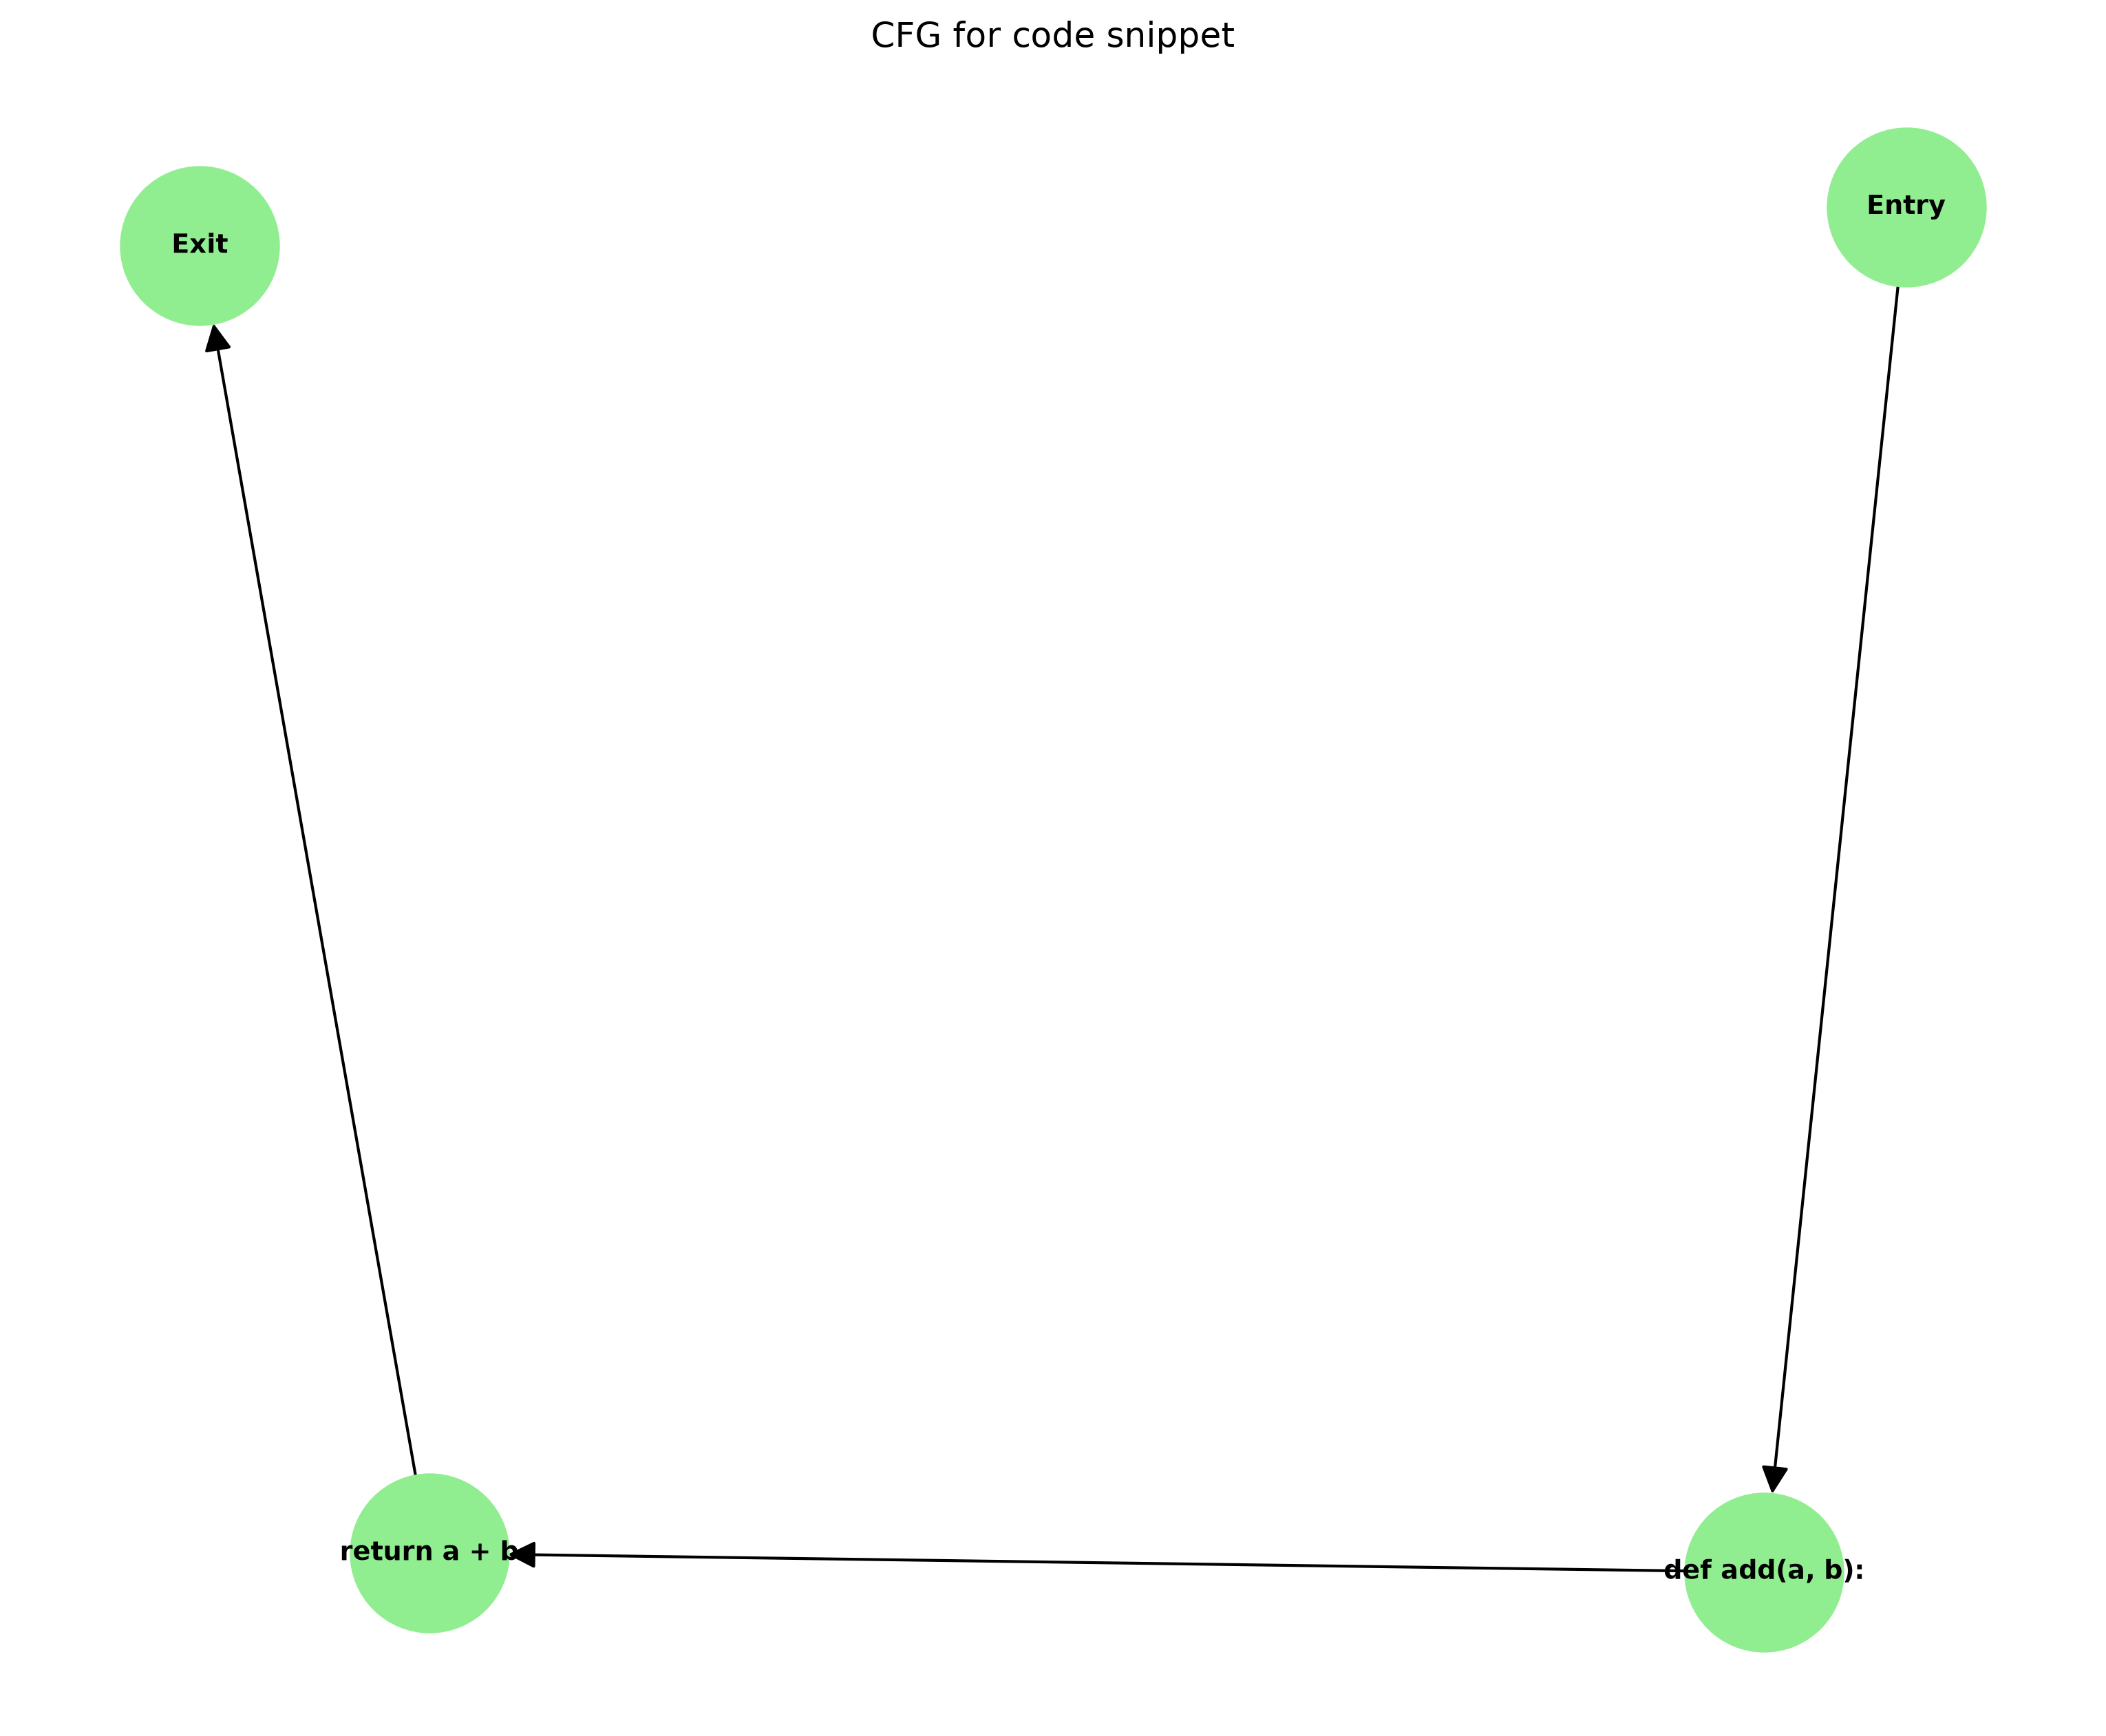
\includegraphics[width=0.8\textwidth]{cfg_sample_1.png}
\caption{CFG for a simple addition function}
\end{figure}

\begin{figure}[h]
\centering
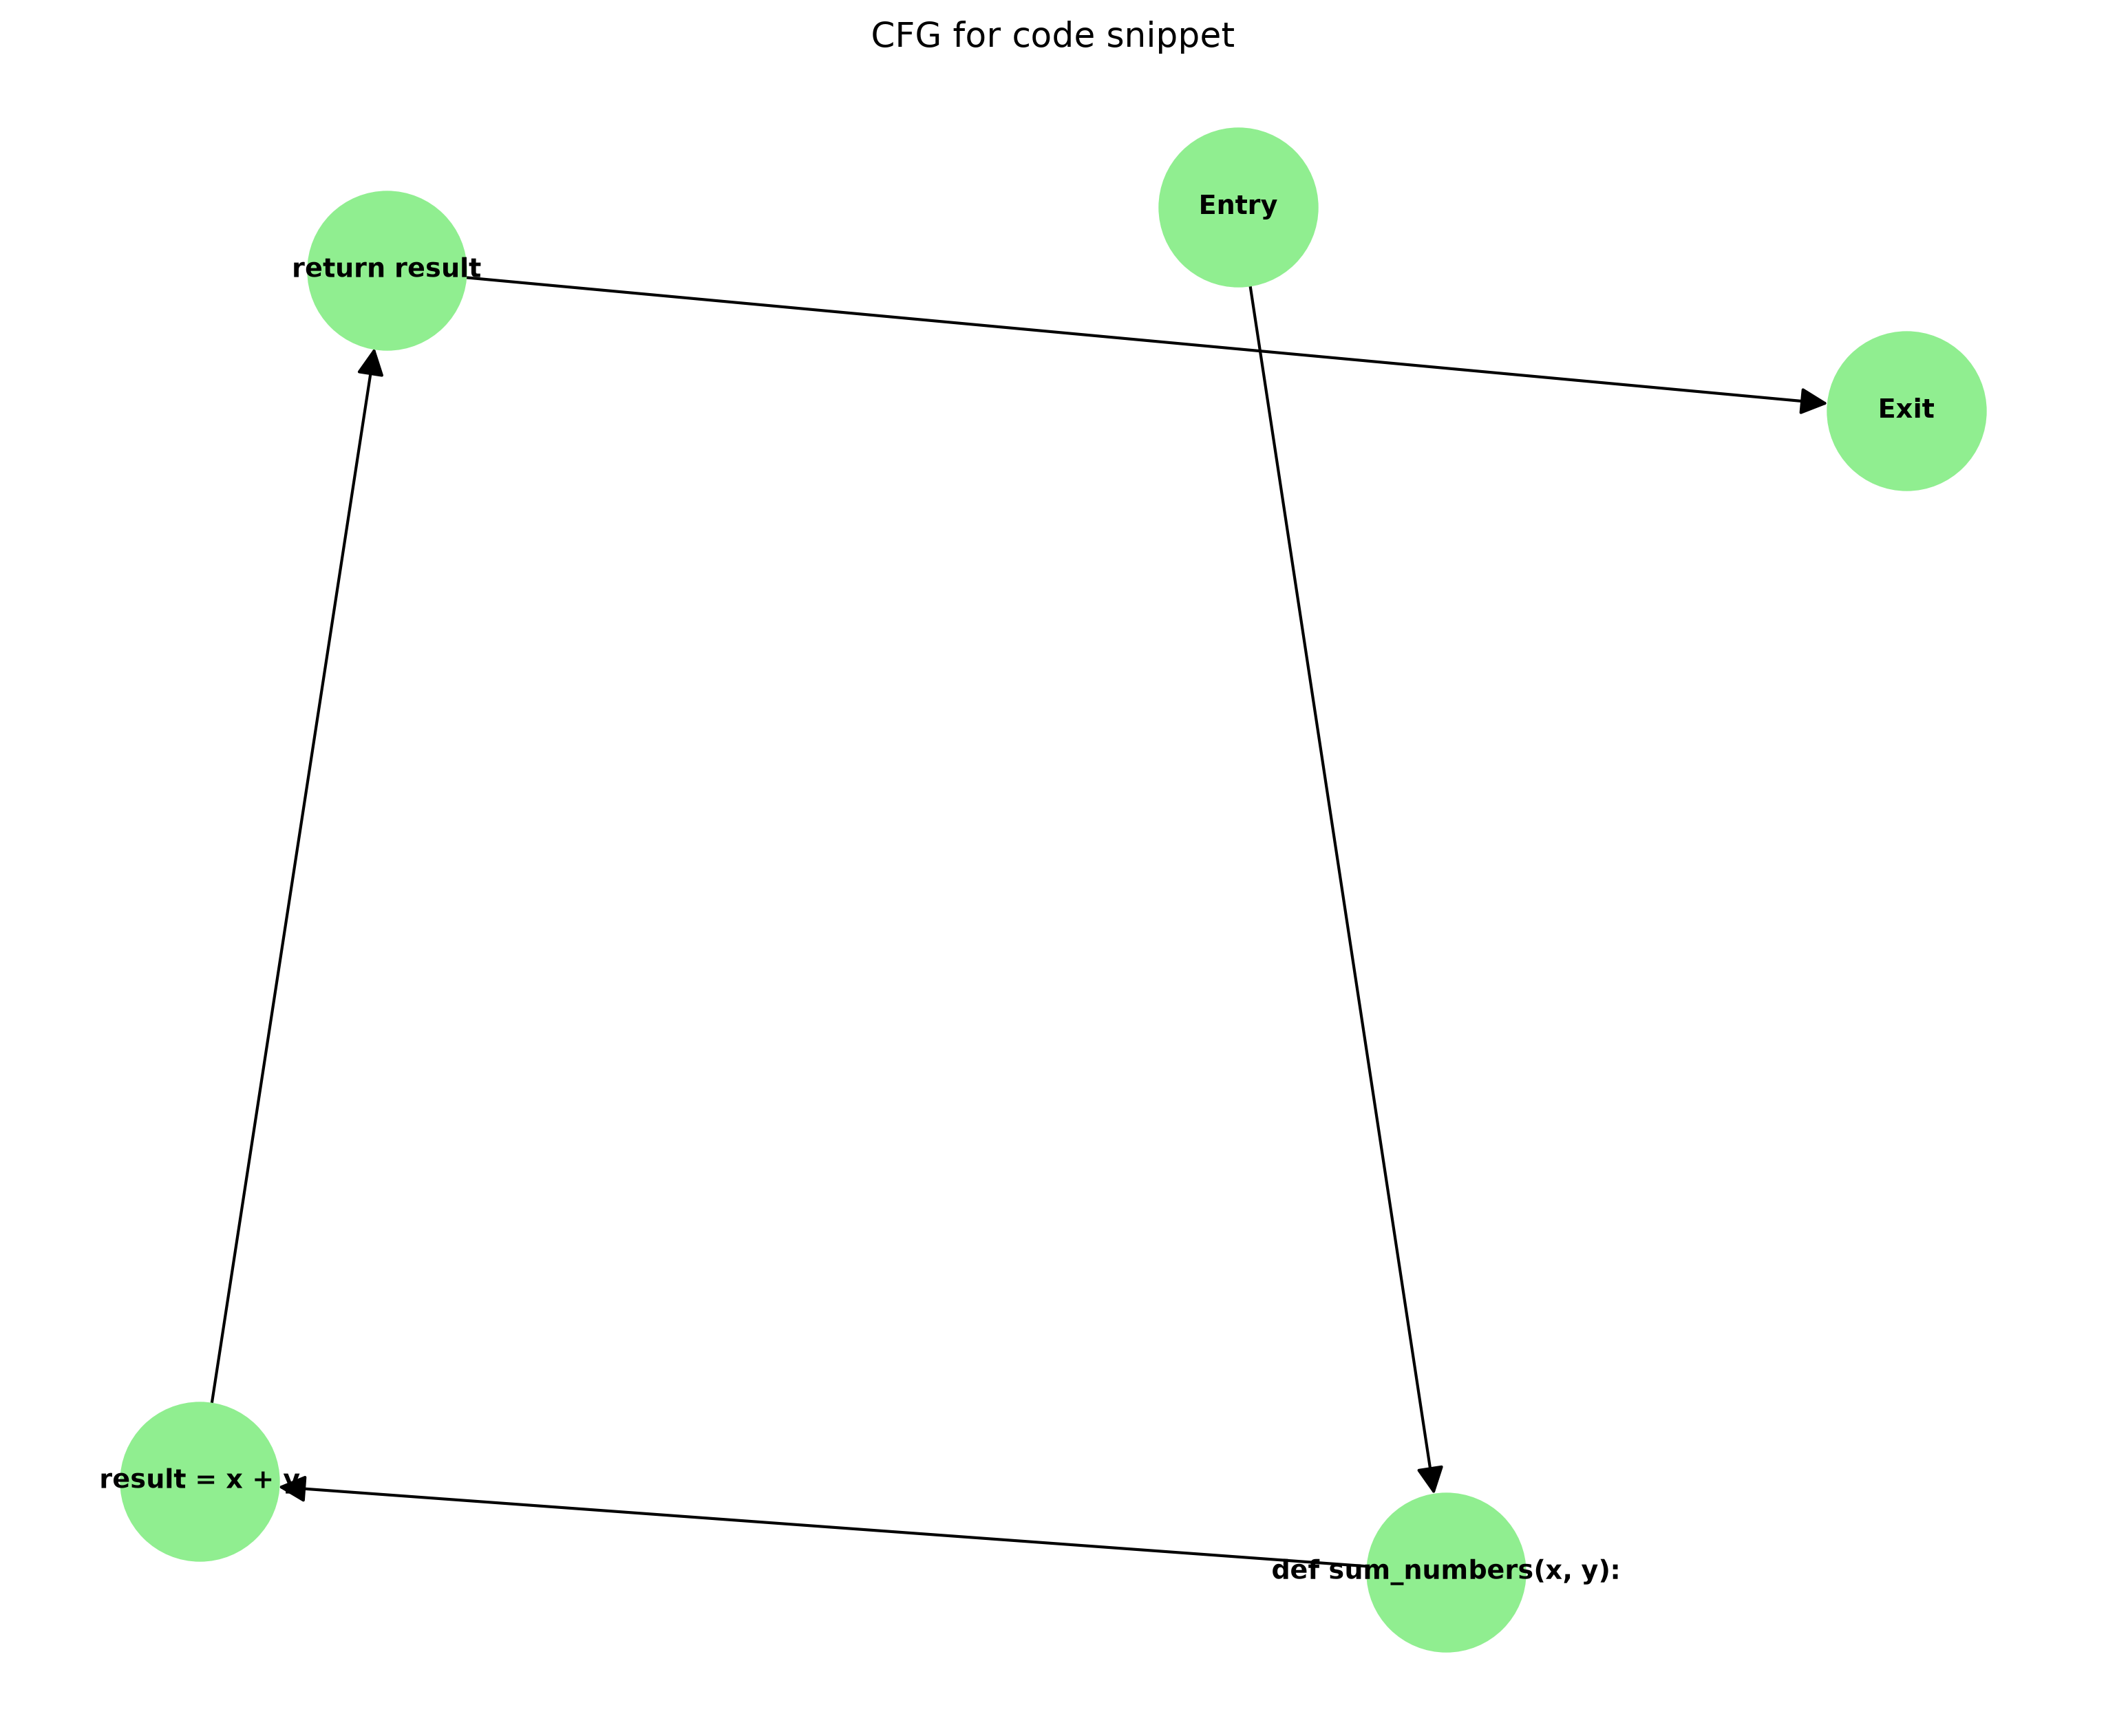
\includegraphics[width=0.8\textwidth]{cfg_sample_2.png}
\caption{CFG for a function with intermediate variable}
\end{figure}

\begin{figure}[h]
\centering
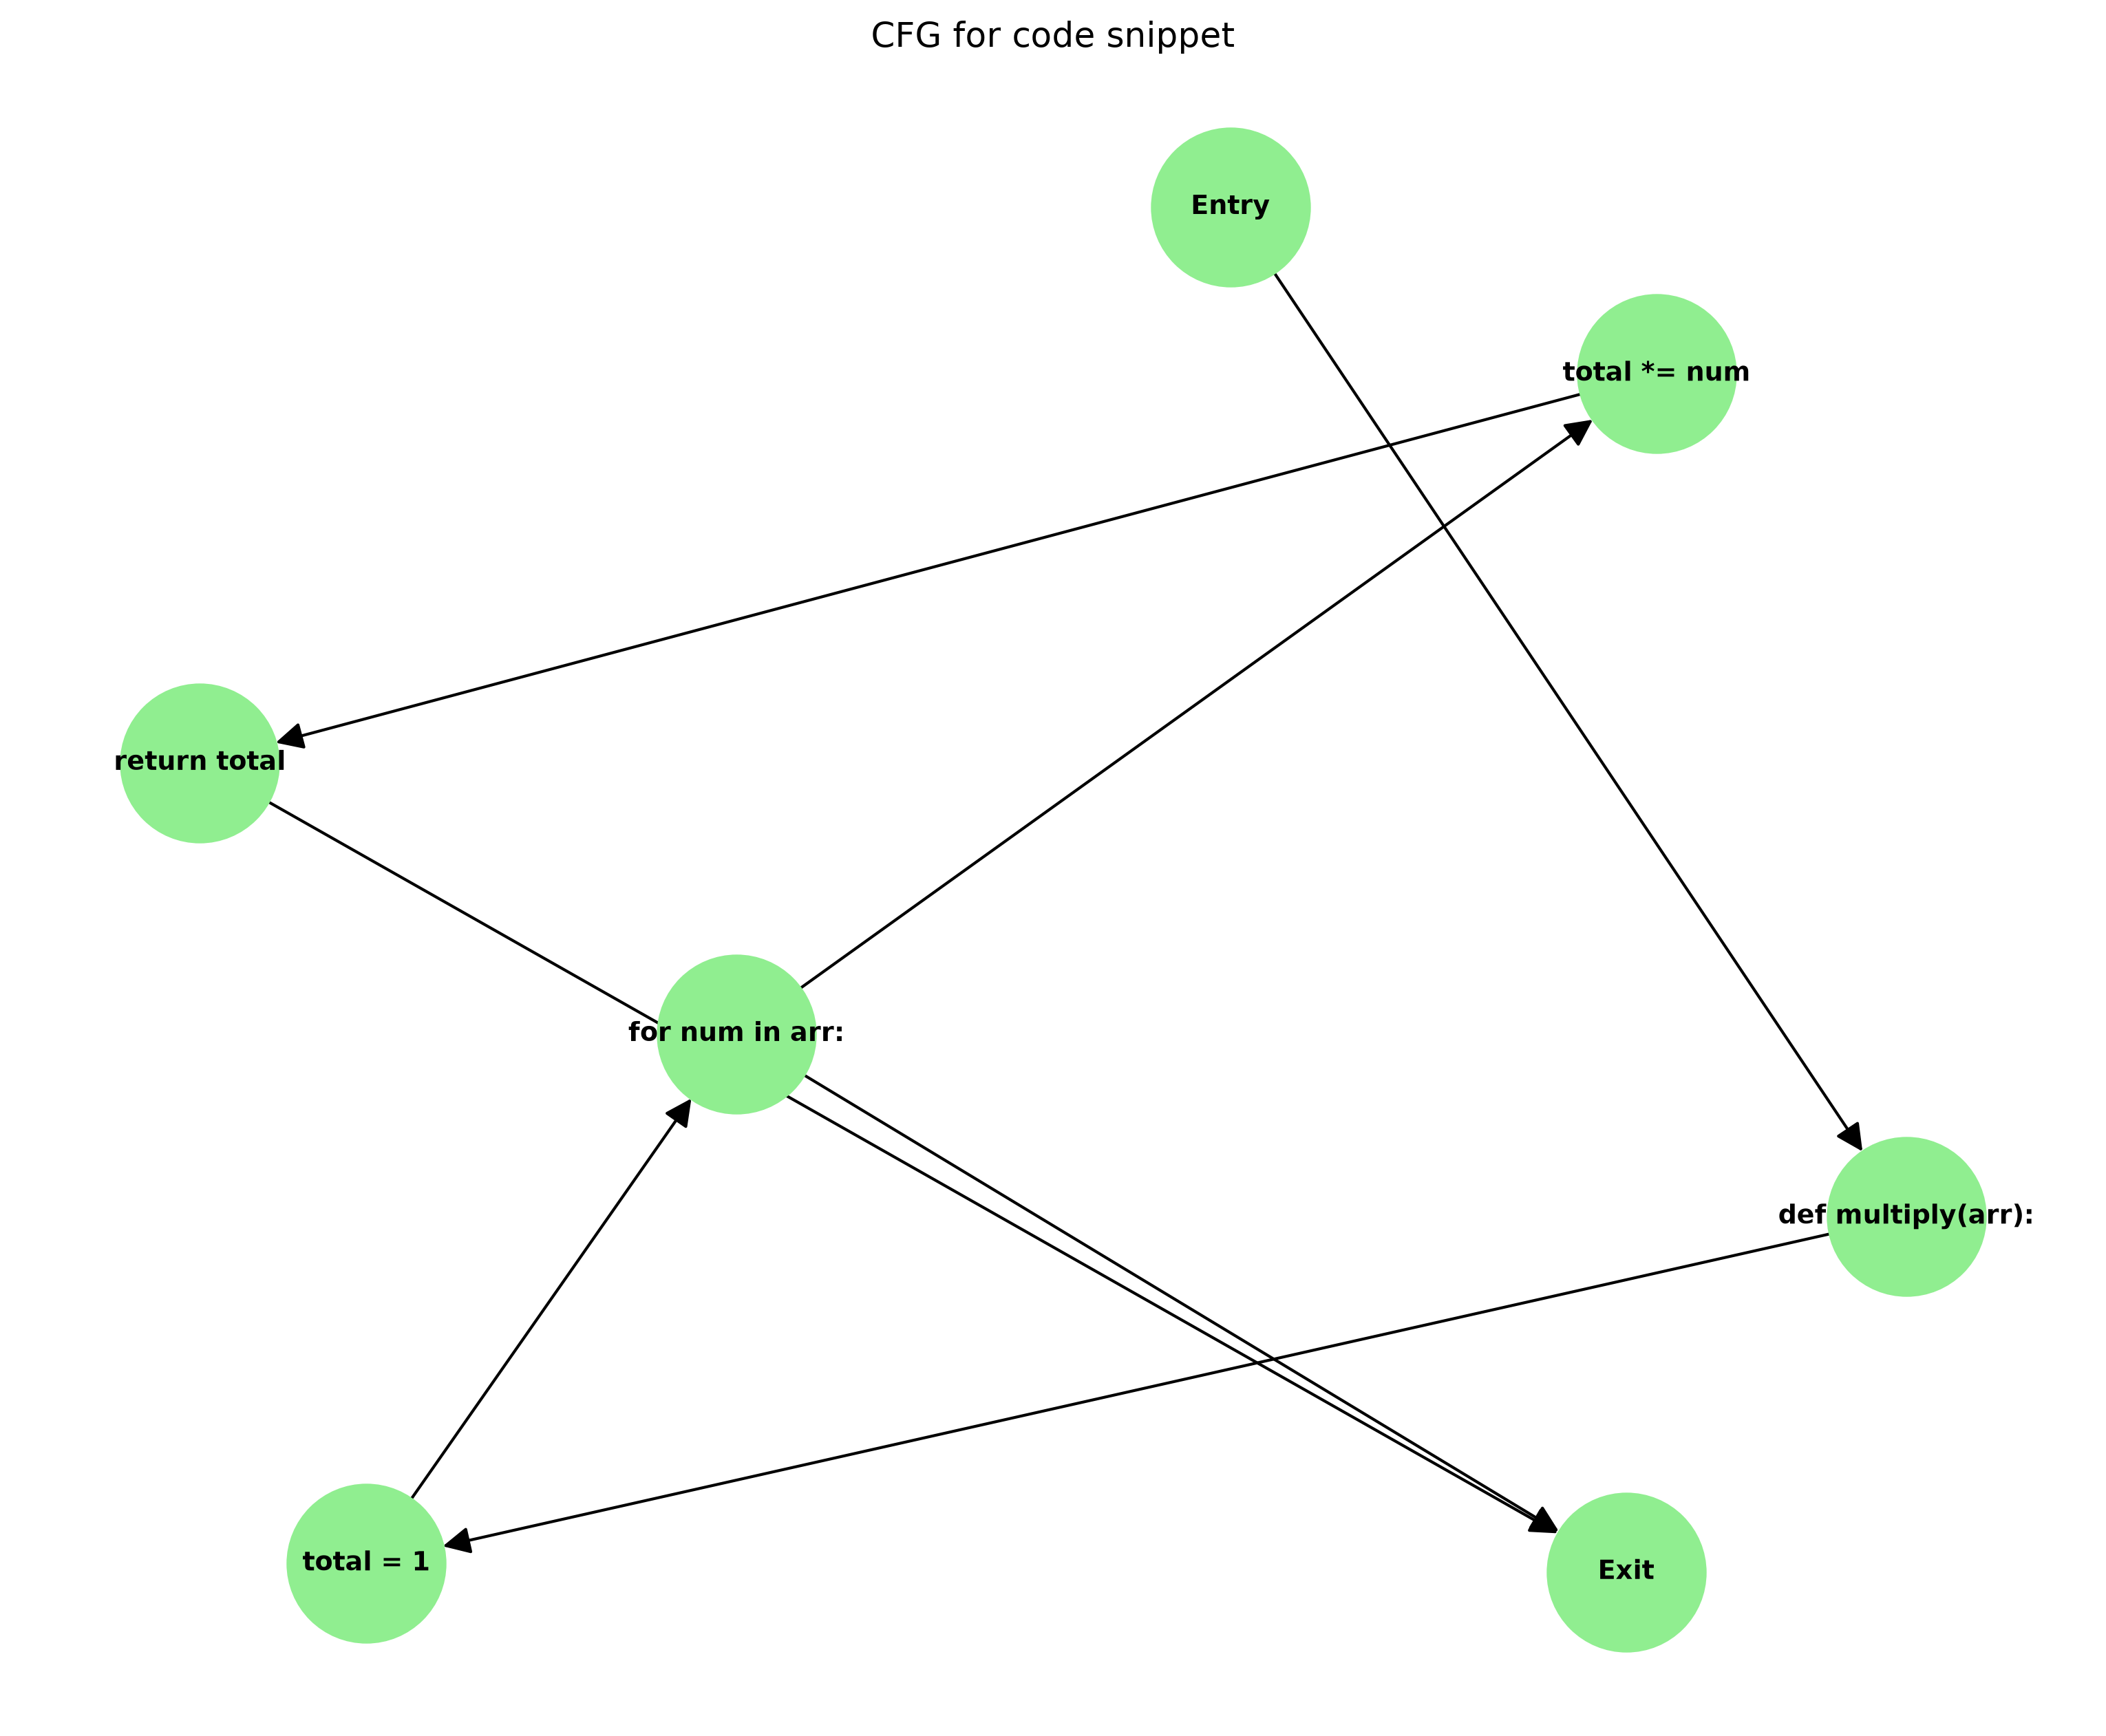
\includegraphics[width=0.8\textwidth]{cfg_sample_3.png}
\caption{CFG for a function with loop}
\end{figure}


\begin{figure}[h]
\centering
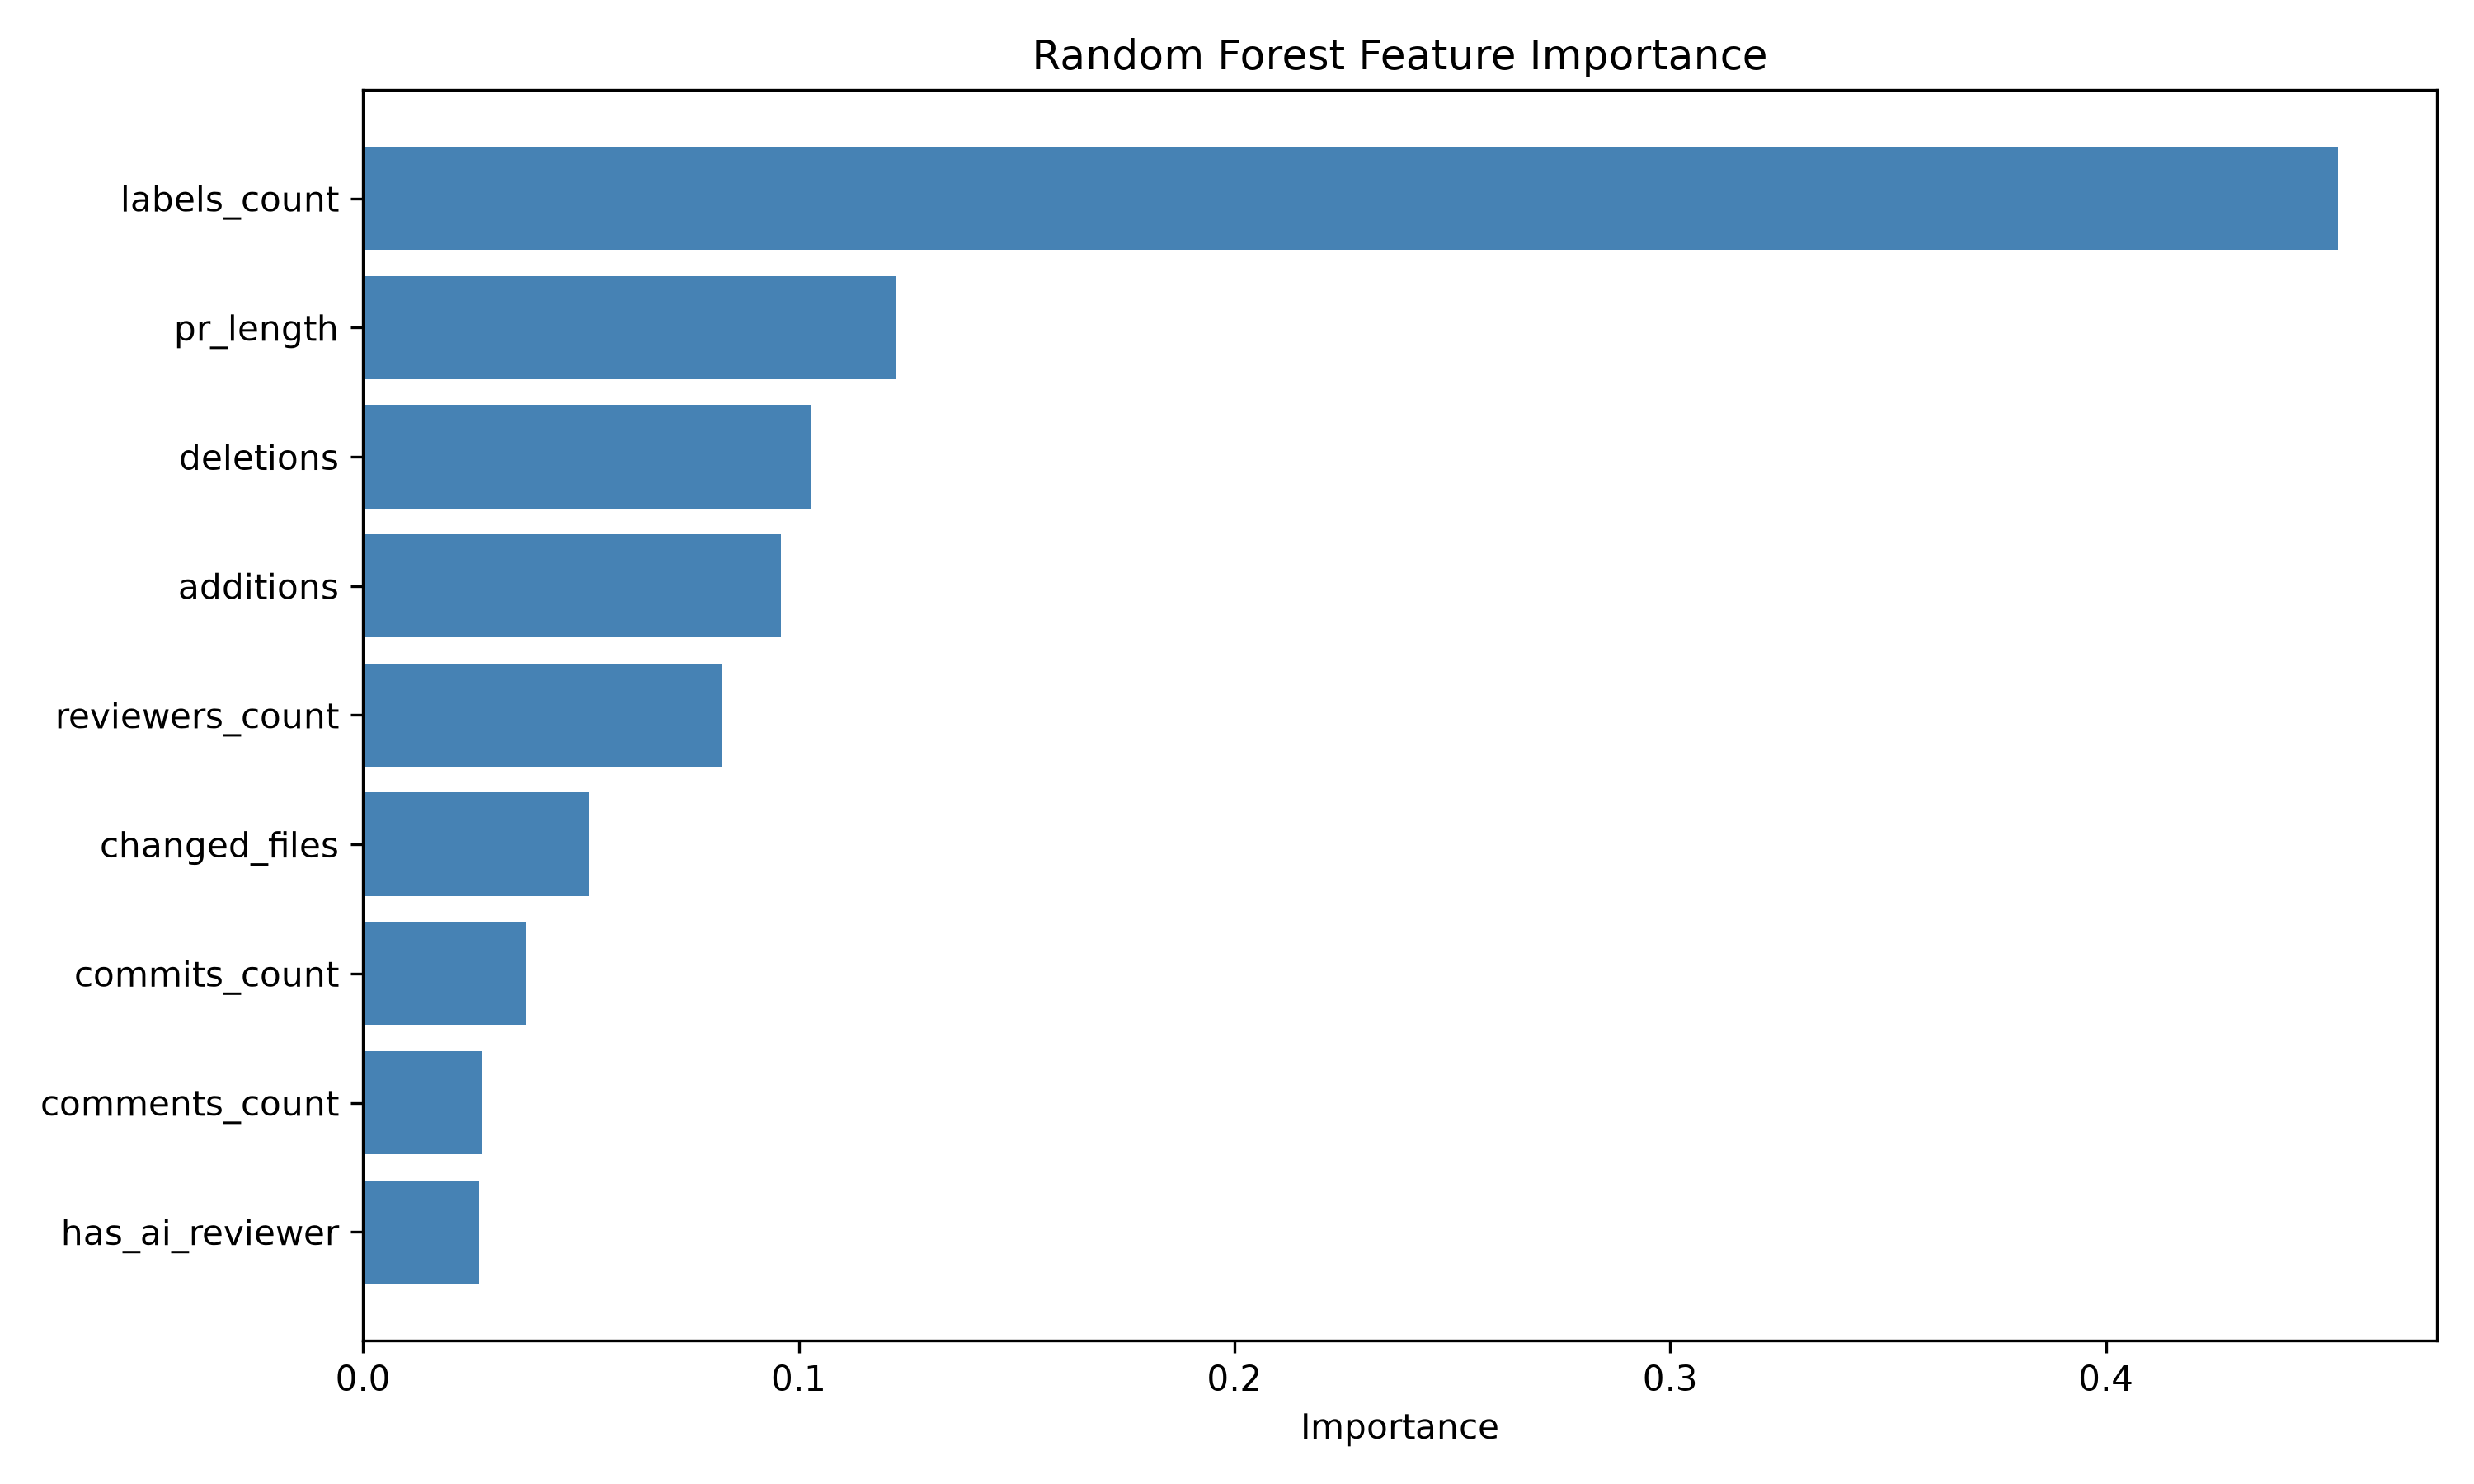
\includegraphics[width=0.8\textwidth]{feature_importance.png}
\caption{Random Forest feature importance}
\end{figure}

\begin{figure}[h]
\centering
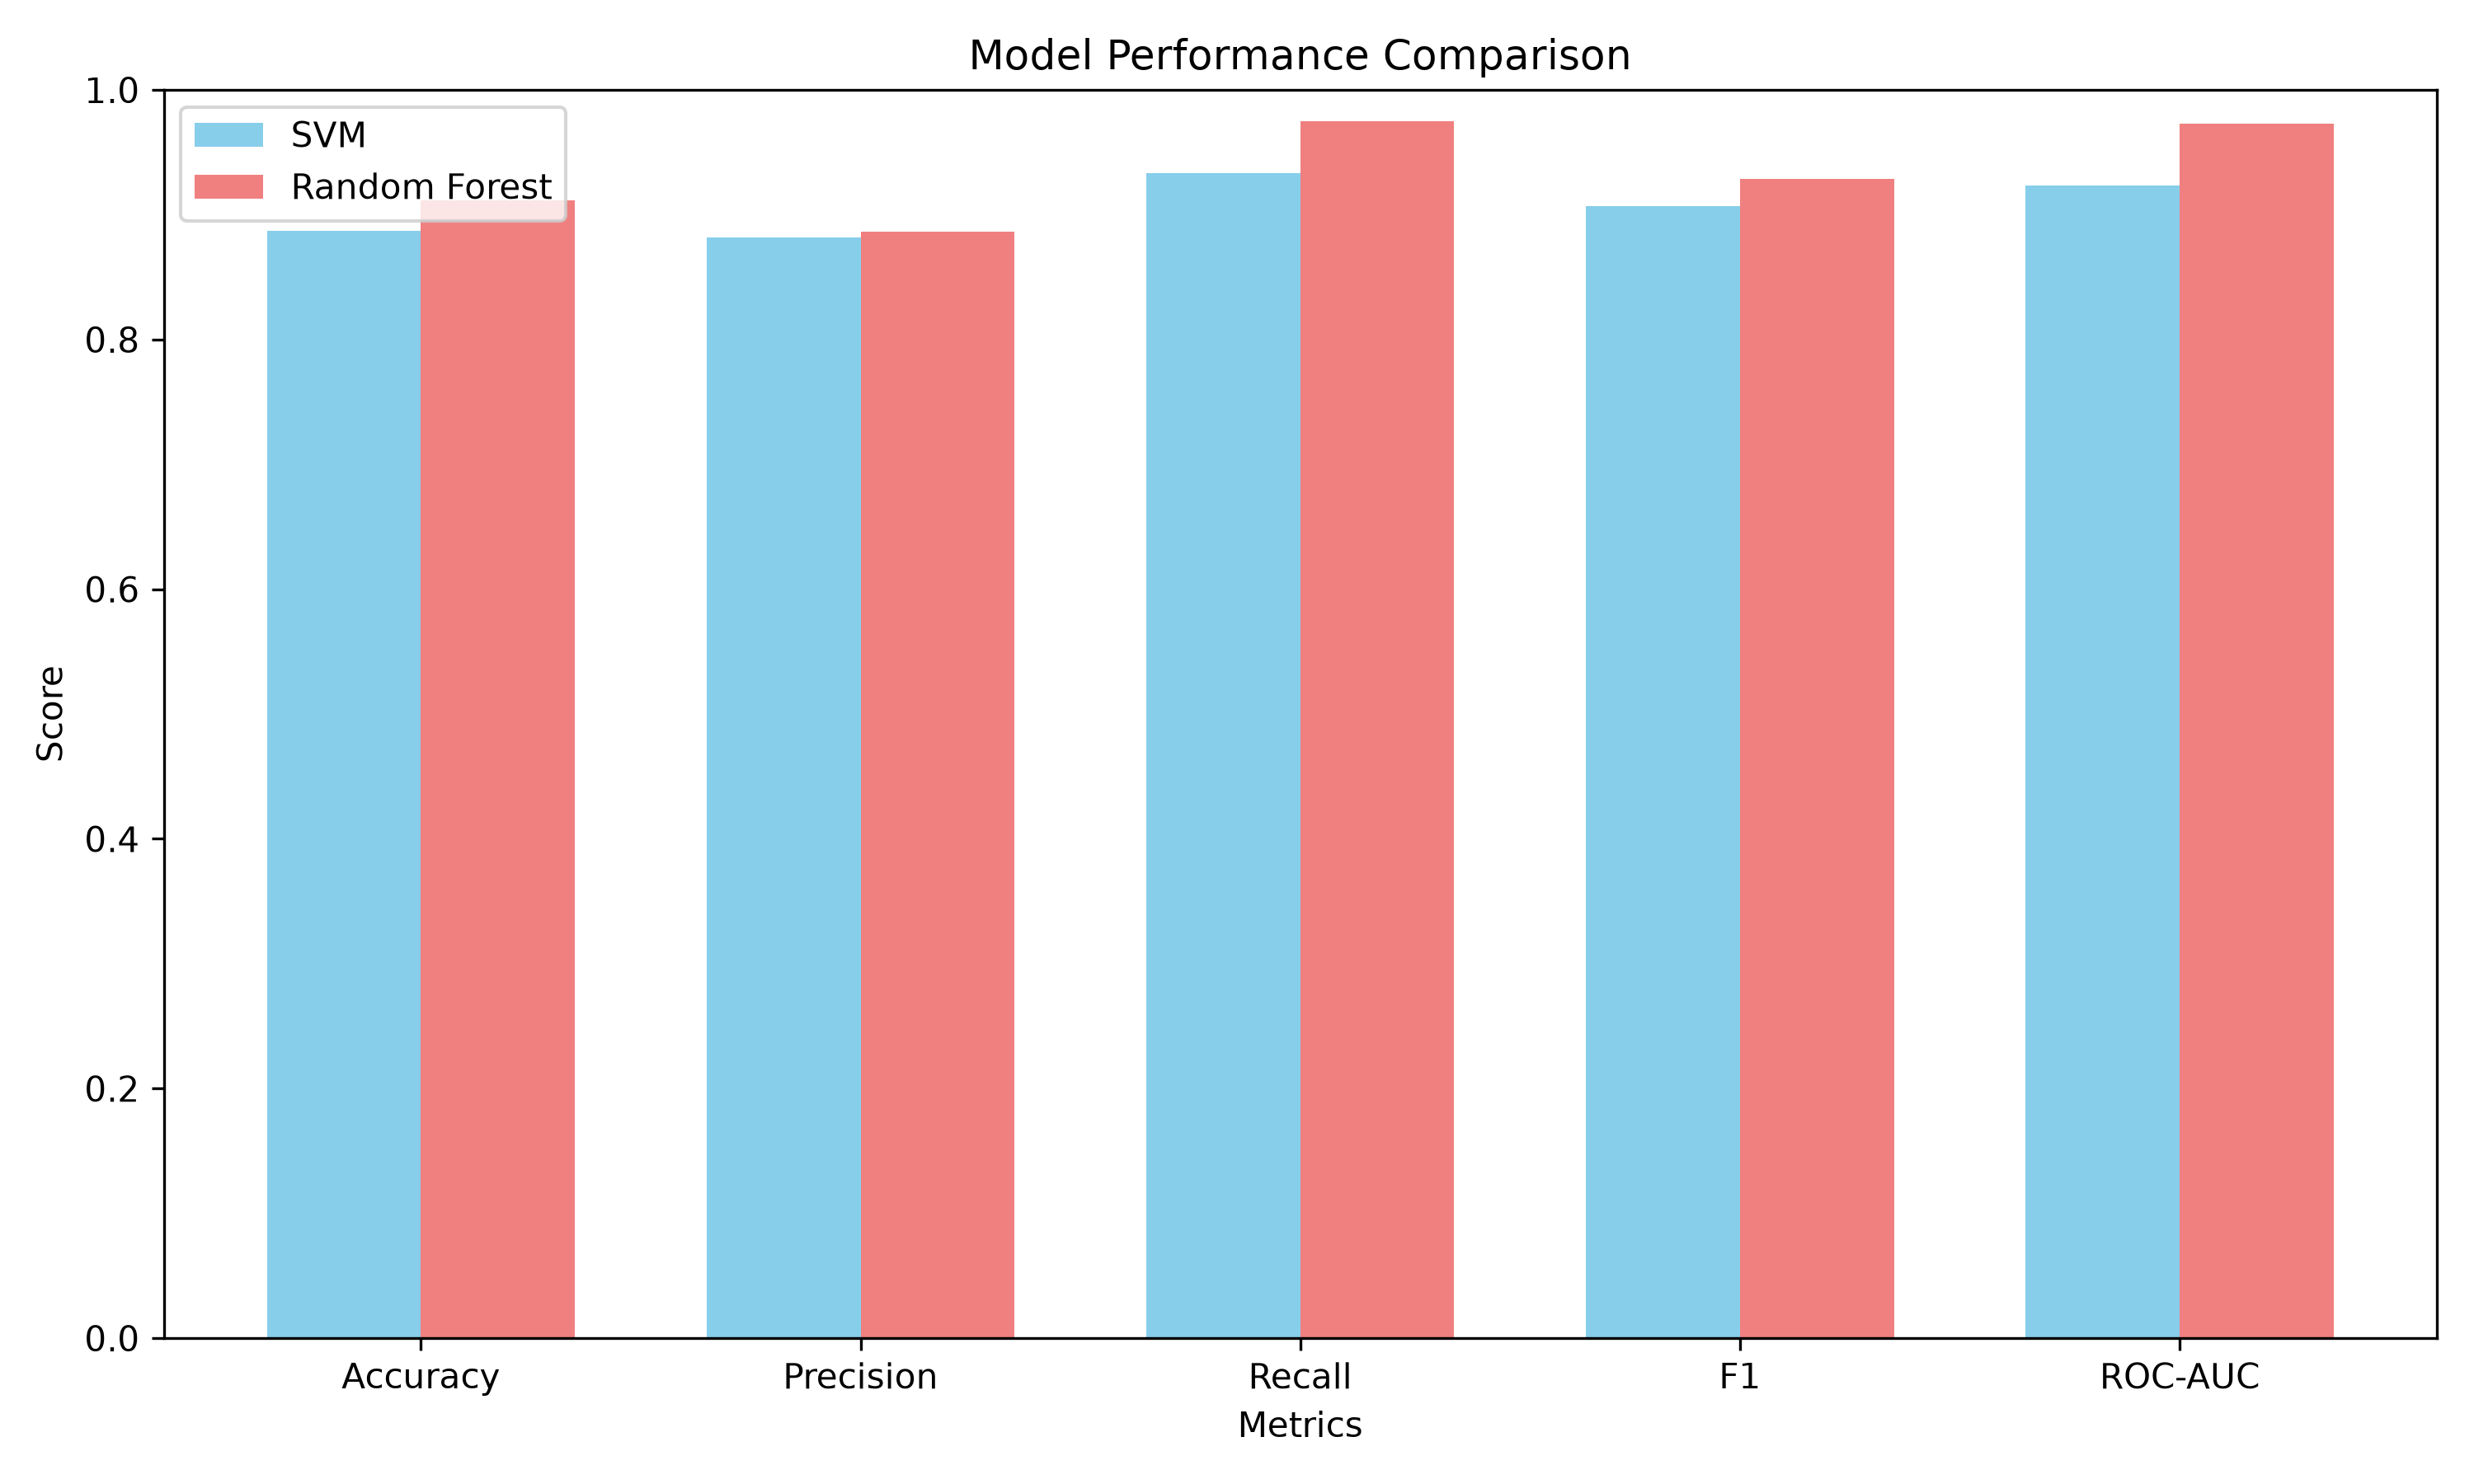
\includegraphics[width=0.8\textwidth]{model_comparison.png}
\caption{SVM vs Random Forest performance comparison}
\end{figure}

\clearpage

\experimentproblems{
- Pandas and scikit-learn missing in venv - installed via pip.
- AST/CFG visualization required networkx - installed separately.
- sklearn package name deprecated - used scikit-learn instead.
}

\experimentexperience{
- AST/CFG capture program semantics that raw text cannot represent, enabling deeper code understanding.
- Traditional ML requires manual feature engineering because algorithms cannot directly interpret code syntax and semantics.
- SVM works well for small datasets with clear separation; Random Forest handles complex interactions and provides feature importance.
- labels\_count was the most important feature - PRs with more labels are better organized and more likely to merge.
- Experiment 2 added feature engineering, scaling, model training, and evaluation to the data collection pipeline.
}


%========================
% Instructor Comments
%========================

\teachercomment

\end{document}